\chapter{Discussion on the systematic uncertainties}
\label{sec:Appendix_Syst}

	Comments and discussions on systematic uncertainties are summarized as follows.
	
	\begin{itemize}
	\item \textbf{Pileup}. The uncertainty in the Cat2 in the $\cPZ$ decay is small compared to other categories. No weird behavior in the pileup weights of all three categories is found, no mistake is made when the pileup weights are evaluated and applied. Table~\ref{tab:UnPUwei} shows the detail numbers that give the final uncertainties in all the categories. Fig.~\ref{fig:puweidiff1D} shows the distributions of the difference between the up (down) variation and the nominal pileup weight of all the three categorizes in the $\cPZ$ decay. Fig.~\ref{fig:puweidiffvsphoR9} shows the 2D distributions of the difference between the up (down) variation and the nominal pile-up weight versus the photon $\RNINE$ value. In Fig.~\ref{fig:puweihistory}, the x-axis is the event number while the y-axis is the difference with respect to the sum of nominal pile-up weight over all events. This plot clearly shows how the difference evolves with the events in each category. As one can see, such small uncertainty in EBLR9 category is due to the cancellation of positive and negative weights.  
 \end{itemize}

	\begin{table}[!ht]
	\scriptsize
	%\setlength{\tabcolsep}{10pt} % Default value: 6pt
	%  \renewcommand{\arraystretch}{2} % Default value: 1
	    \begin{center}
	    \begin{tabular}{lccccccc}
	    \hline
	    & \color{blue} [1] & \color{blue} [2] & fraction \color{blue} [1]/\color{blue} [2] \color{black} (in \%) & \color{blue} [3] & \color{blue} [4] & \color{blue} [5] & Uncertainty (in \%)\\
	    \cline{2-8}
	      EBHR9 & 4423 & 5447 & 44.8 & 589.0 & -687.3 & 10050.1 & -0.98 \\
	      EBLR9 & 2898 & 3257 & 47.1 & 387.2 & -399.7 & 6213.0 & -0.20 \\
	      EE & 1800 & 2287 & 44.0 & 234.7 & -290.9 & 4196.7 & -1.34\\
	      \hline
	      & \color{red} [1] & \color{red} [2] & fraction \color{red} [1]/\color{red} [2] \color{black} (in \%) & \color{red} [3] & \color{red} [4] & \color{red} [5] & Uncertainty (in \%) \\
	    \cline{2-8}
	      EBHR9 & 4956 & 4914 & 50.2 & 728.8 & -629.1 & 10050.1 & 0.99 \\
	      EBLR9 & 2910 & 3245 & 47.3 & 418.6 & -413.0 & 6213.0 & 0.091 \\
	      EE & 2074 & 2013 & 50.7 & 307.9 & -254.1 & 4196.7 & 1.28\\
	      \hline
	    \multicolumn{8}{l}{[1]: number of events where (puwei\_\color{blue}up\color{black}/\color{red}down \color{black} - puwei)$>0$} \\
	    \multicolumn{8}{l}{[2]: number of events where (puwei\_\color{blue}up\color{black}/\color{red}down \color{black} - puwei)$<0$}\\
	    \multicolumn{8}{l}{[3]: sum over positive value of (puwei\_\color{blue}up\color{black}/\color{red}down \color{black} - puwei)}\\
	    \multicolumn{8}{l}{[4]: sum over negative value of (puwei\_\color{blue}up\color{black}/\color{red}down \color{black} - puwei)}\\
	    \multicolumn{8}{l}{[5]: sum over all puwei}\\
	    \hline
	    \end{tabular}
	    \bigskip
	    \caption{The uncertainties in pile-up weight of each category. }
	    \label{tab:UnPUwei}
	    \end{center}
	\end{table} 
 
 \begin{figure}[!ht]
	  \begin{center}
	    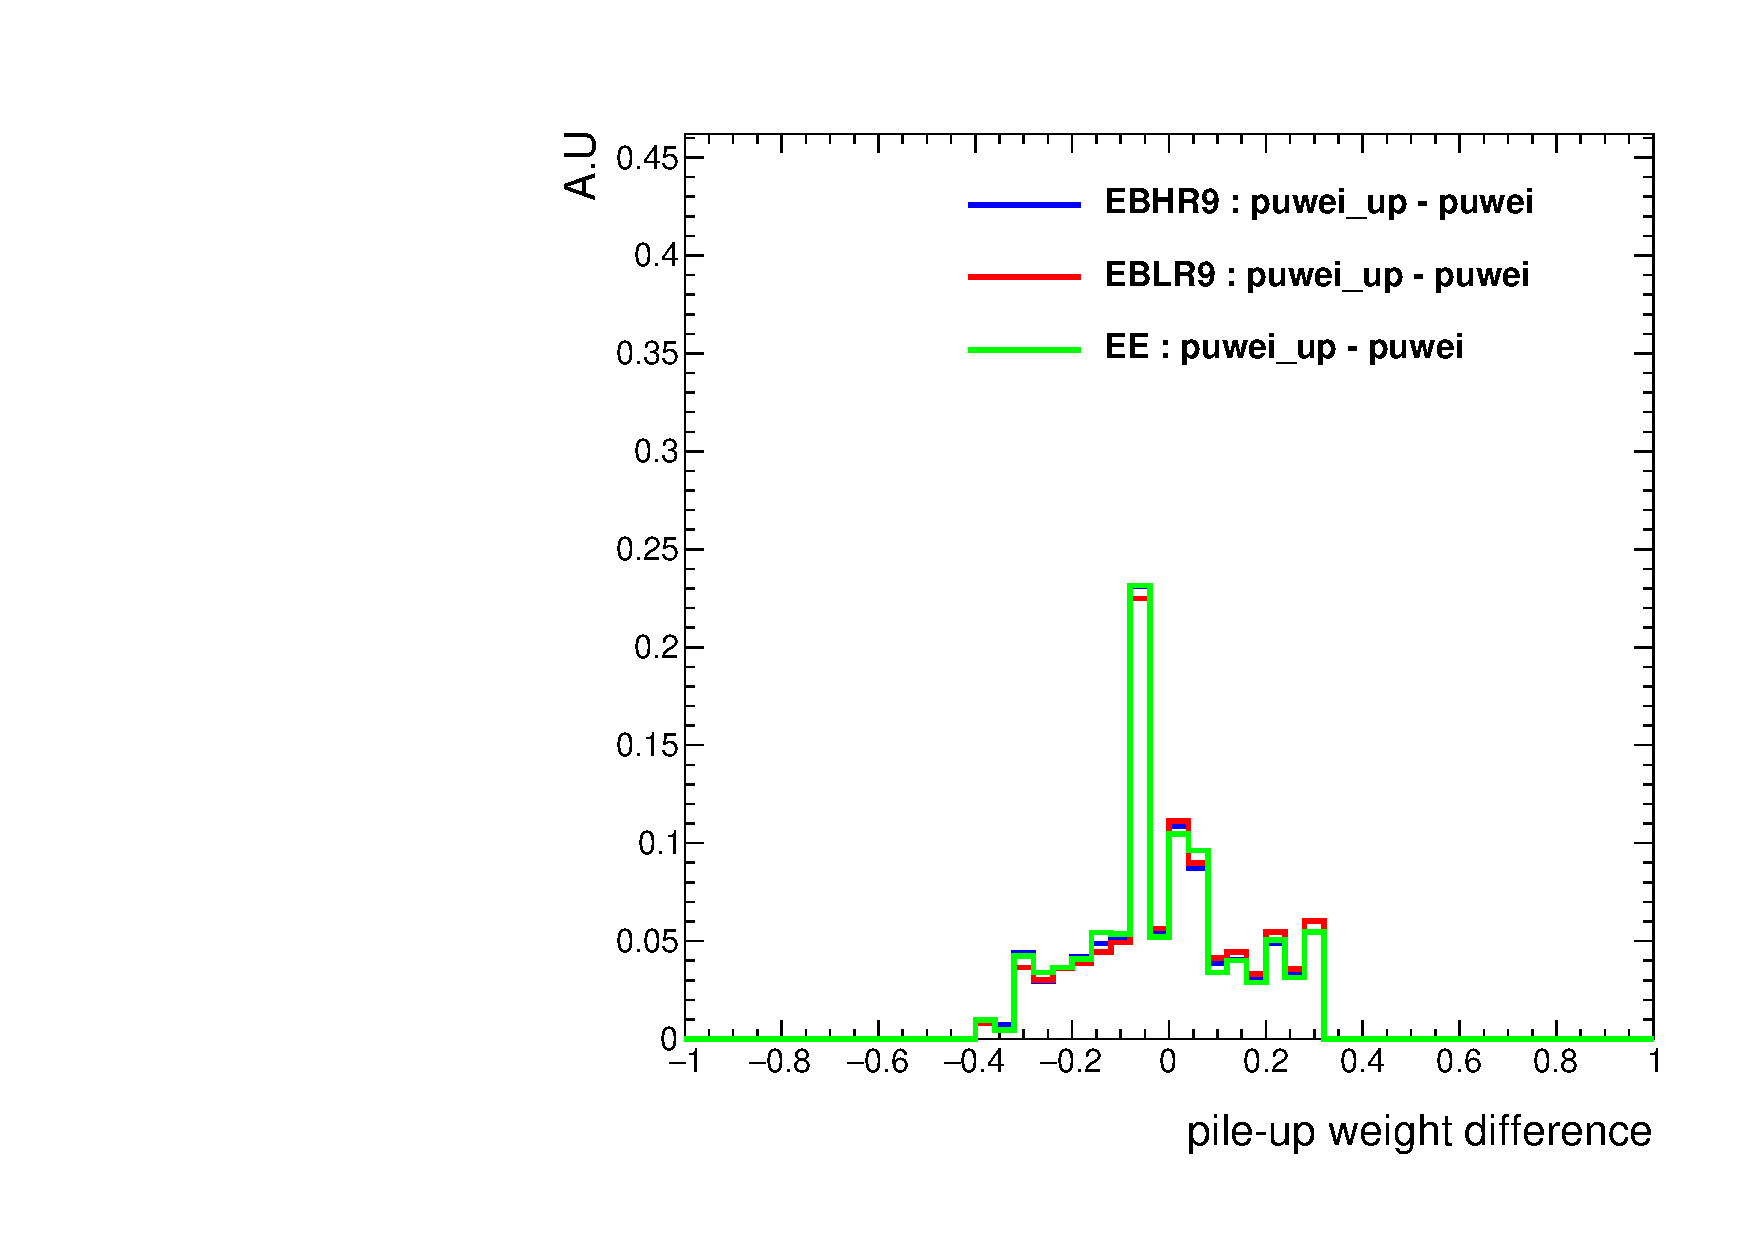
\includegraphics[width=0.50\textwidth]{Fig/puwei_check/puweiup_diff}~
	    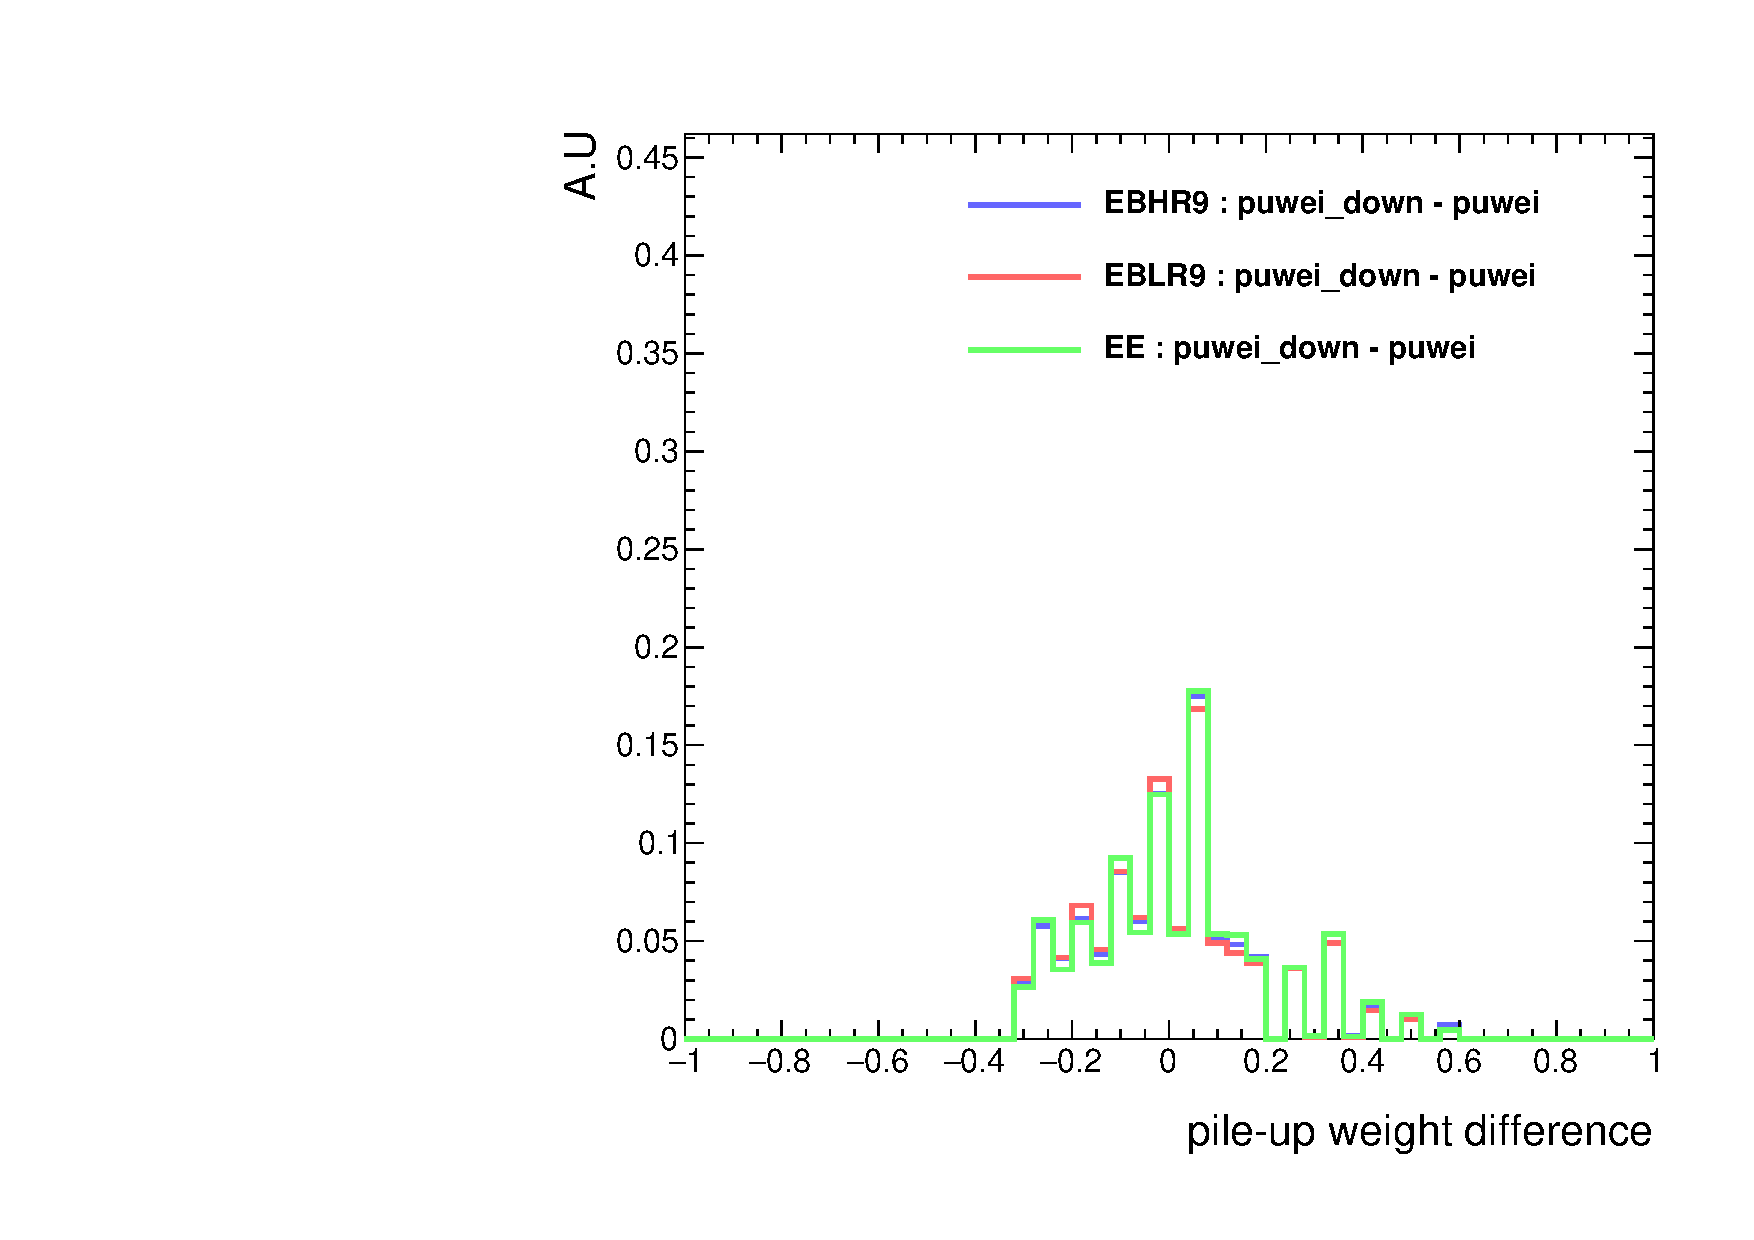
\includegraphics[width=0.50\textwidth]{Fig/puwei_check/puweidown_diff}\\
	    \bigskip
	    \caption{The 1D distributions of the difference between the up(down) variation and the nominal pile-up weight of all the 3 categorizes in the Z decay.}
	  \label{fig:puweidiff1D}
	  \end{center}
	    \end{figure}
	
	\begin{figure}[p]
	  \begin{center}
	    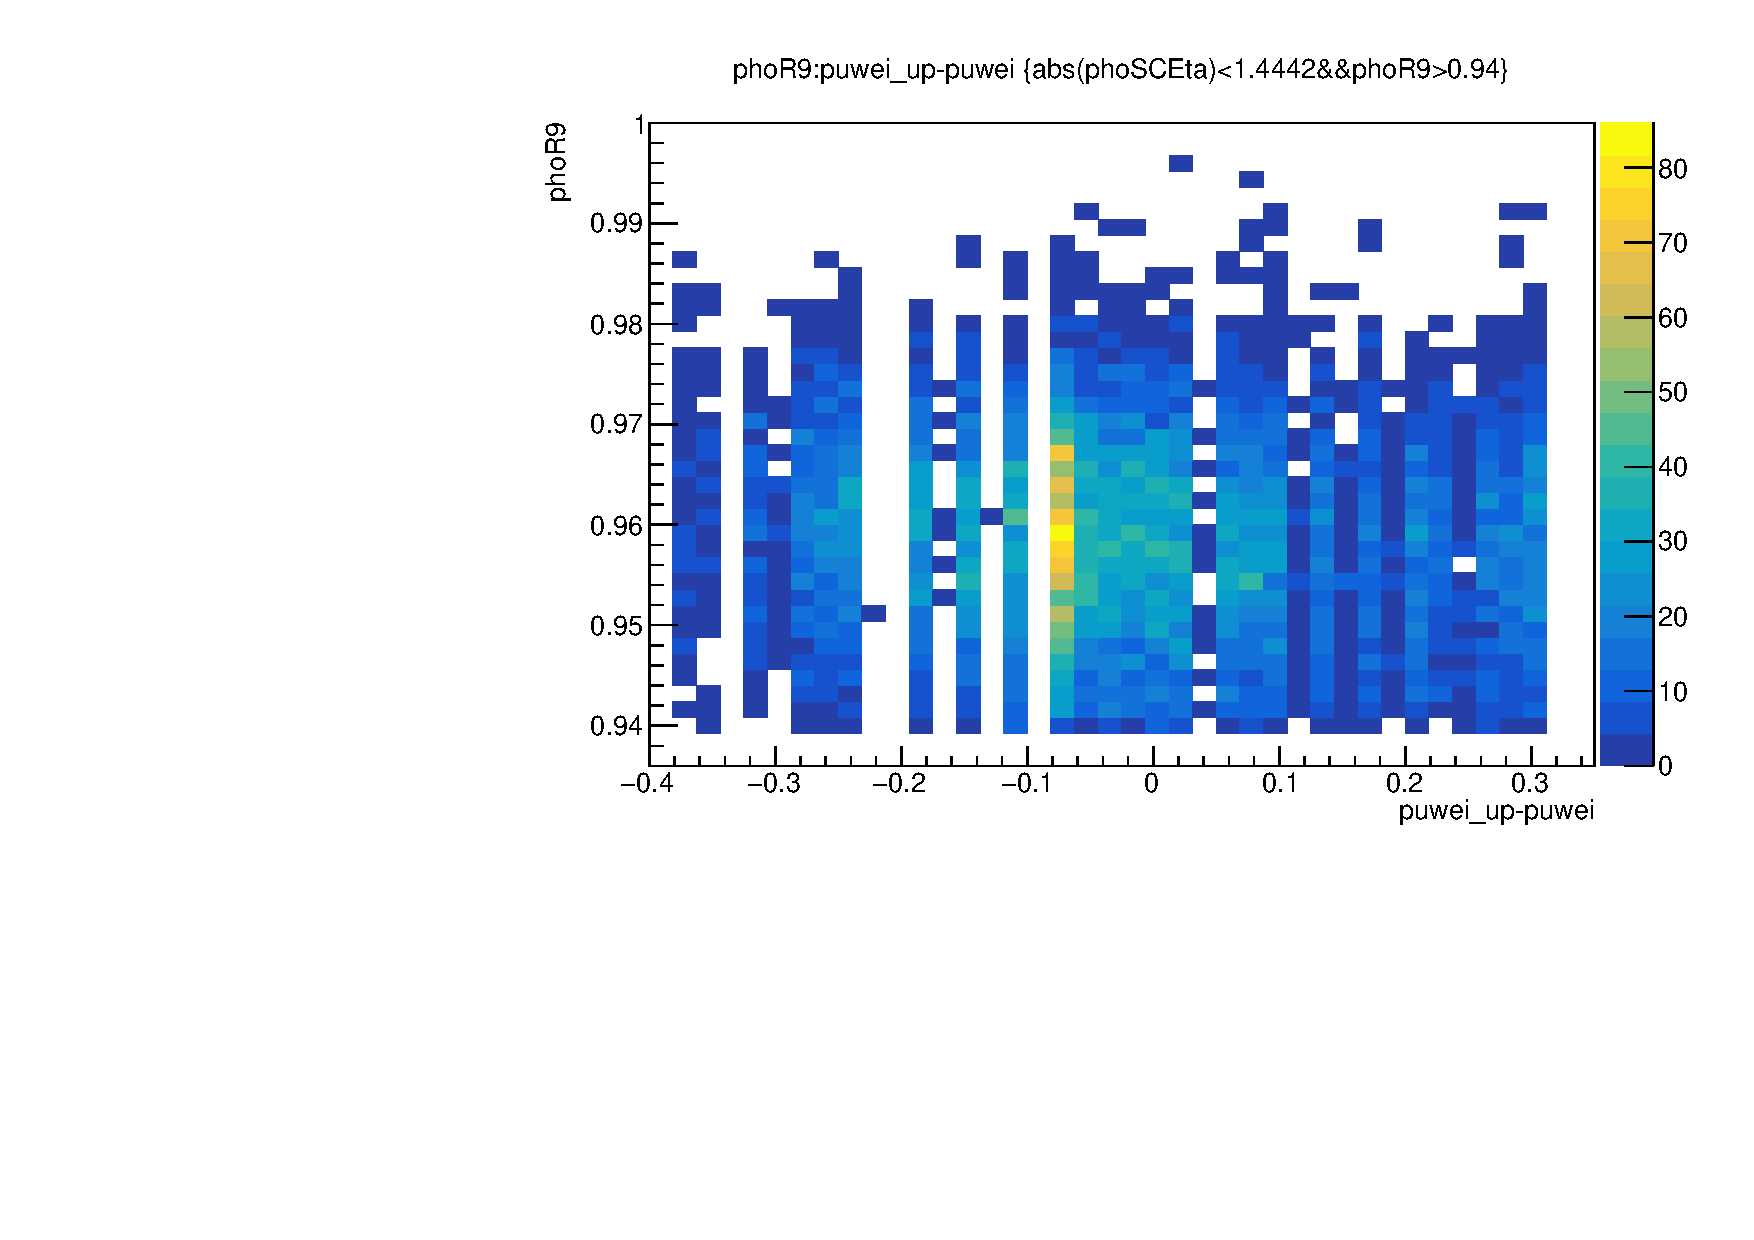
\includegraphics[width=0.50\textwidth]{Fig/puwei_check/phoR9VSpuweiupdiff_EBHR9}~
	    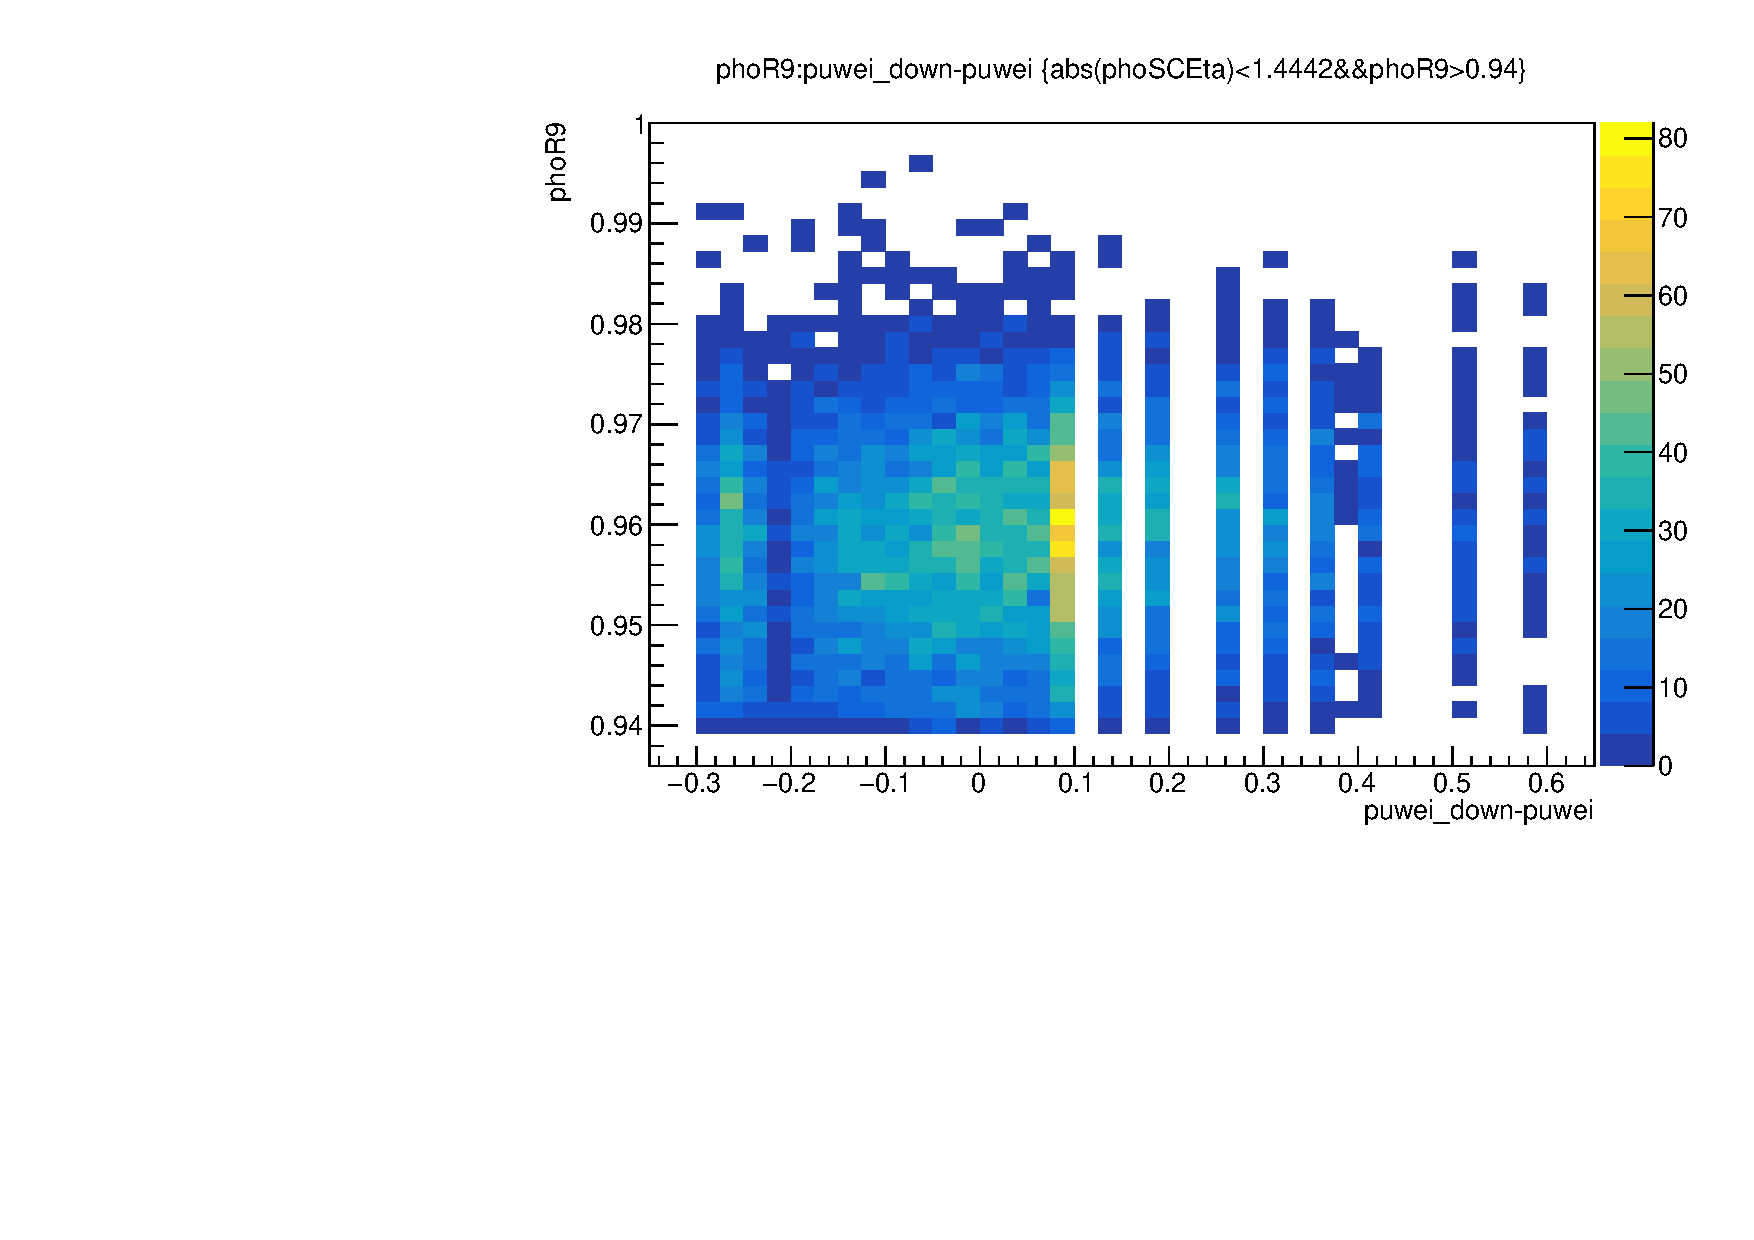
\includegraphics[width=0.50\textwidth]{Fig/puwei_check/phoR9VSpuweidowndiff_EBHR9}\\
	    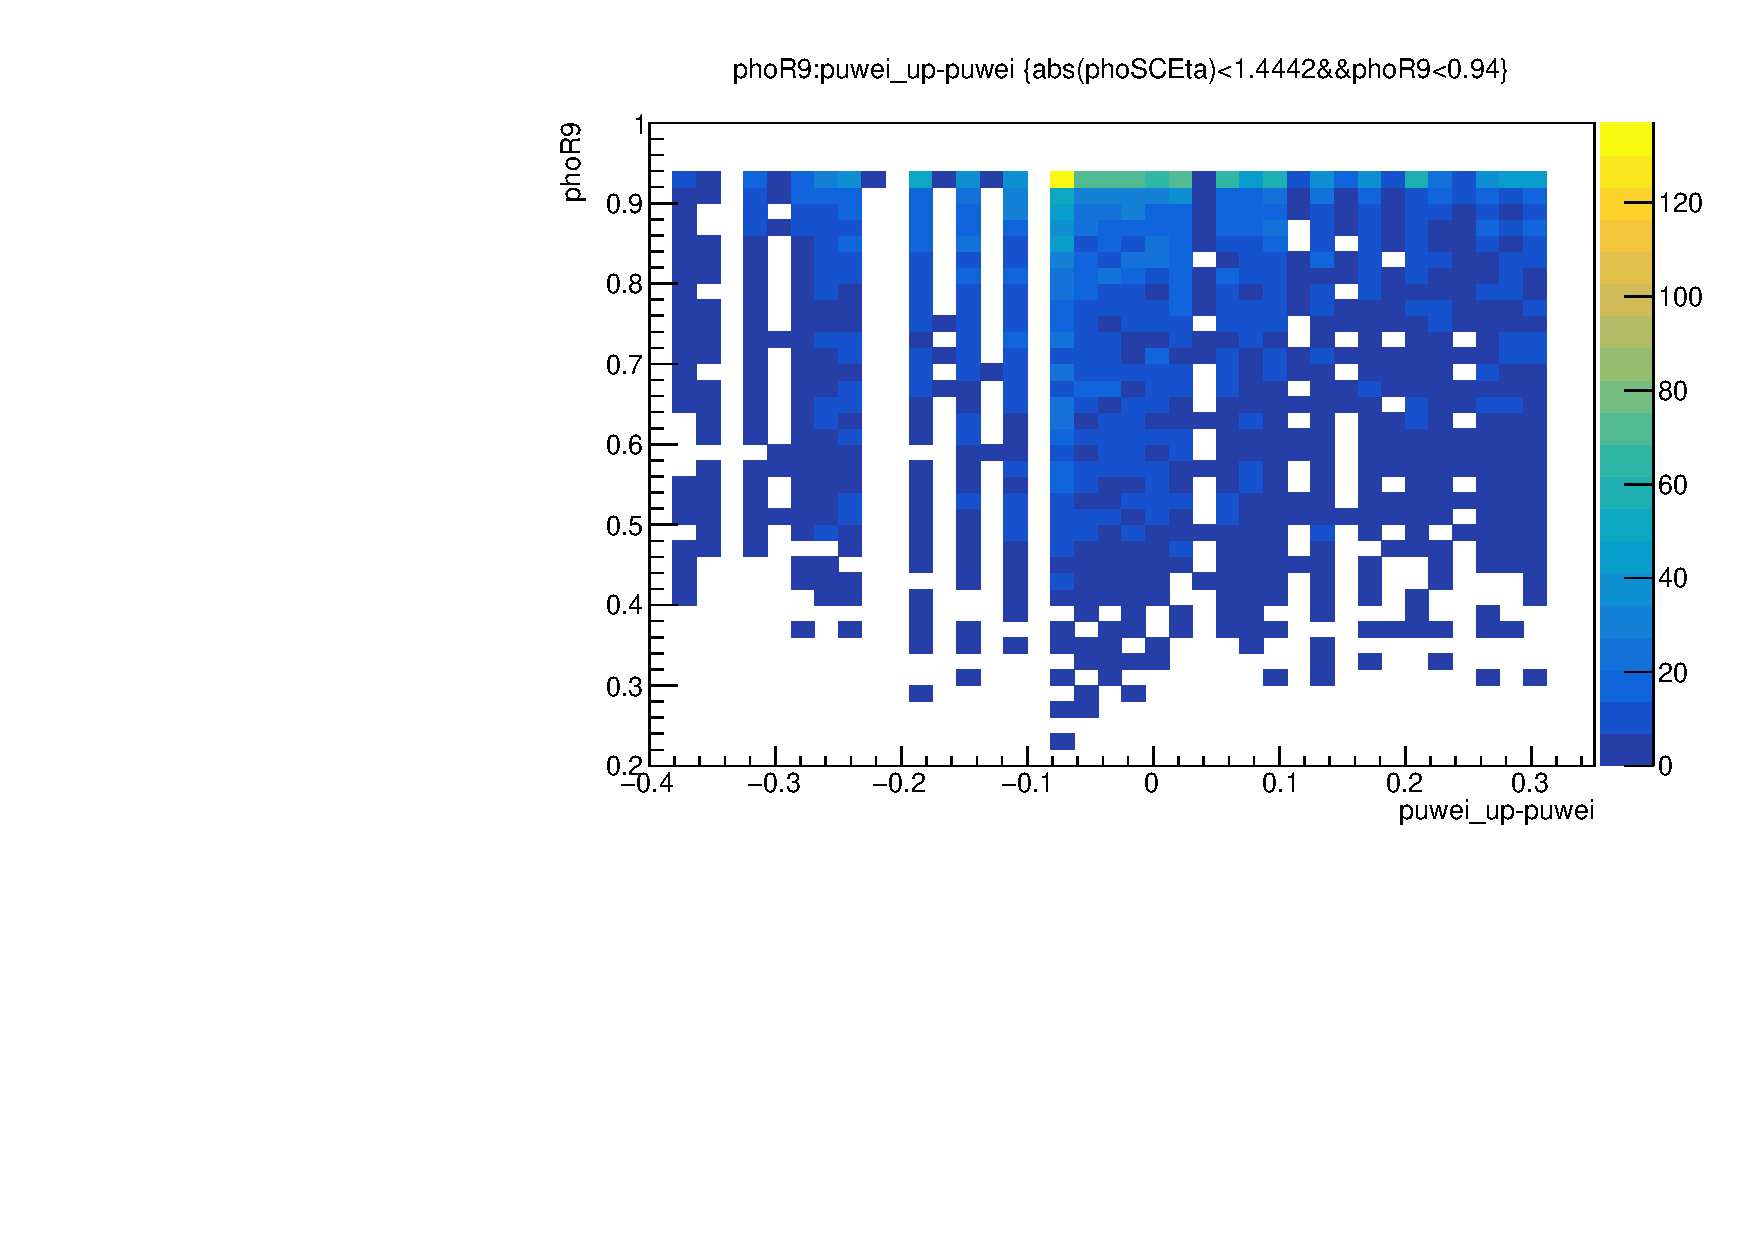
\includegraphics[width=0.50\textwidth]{Fig/puwei_check/phoR9VSpuweiupdiff_EBLR9}~
	    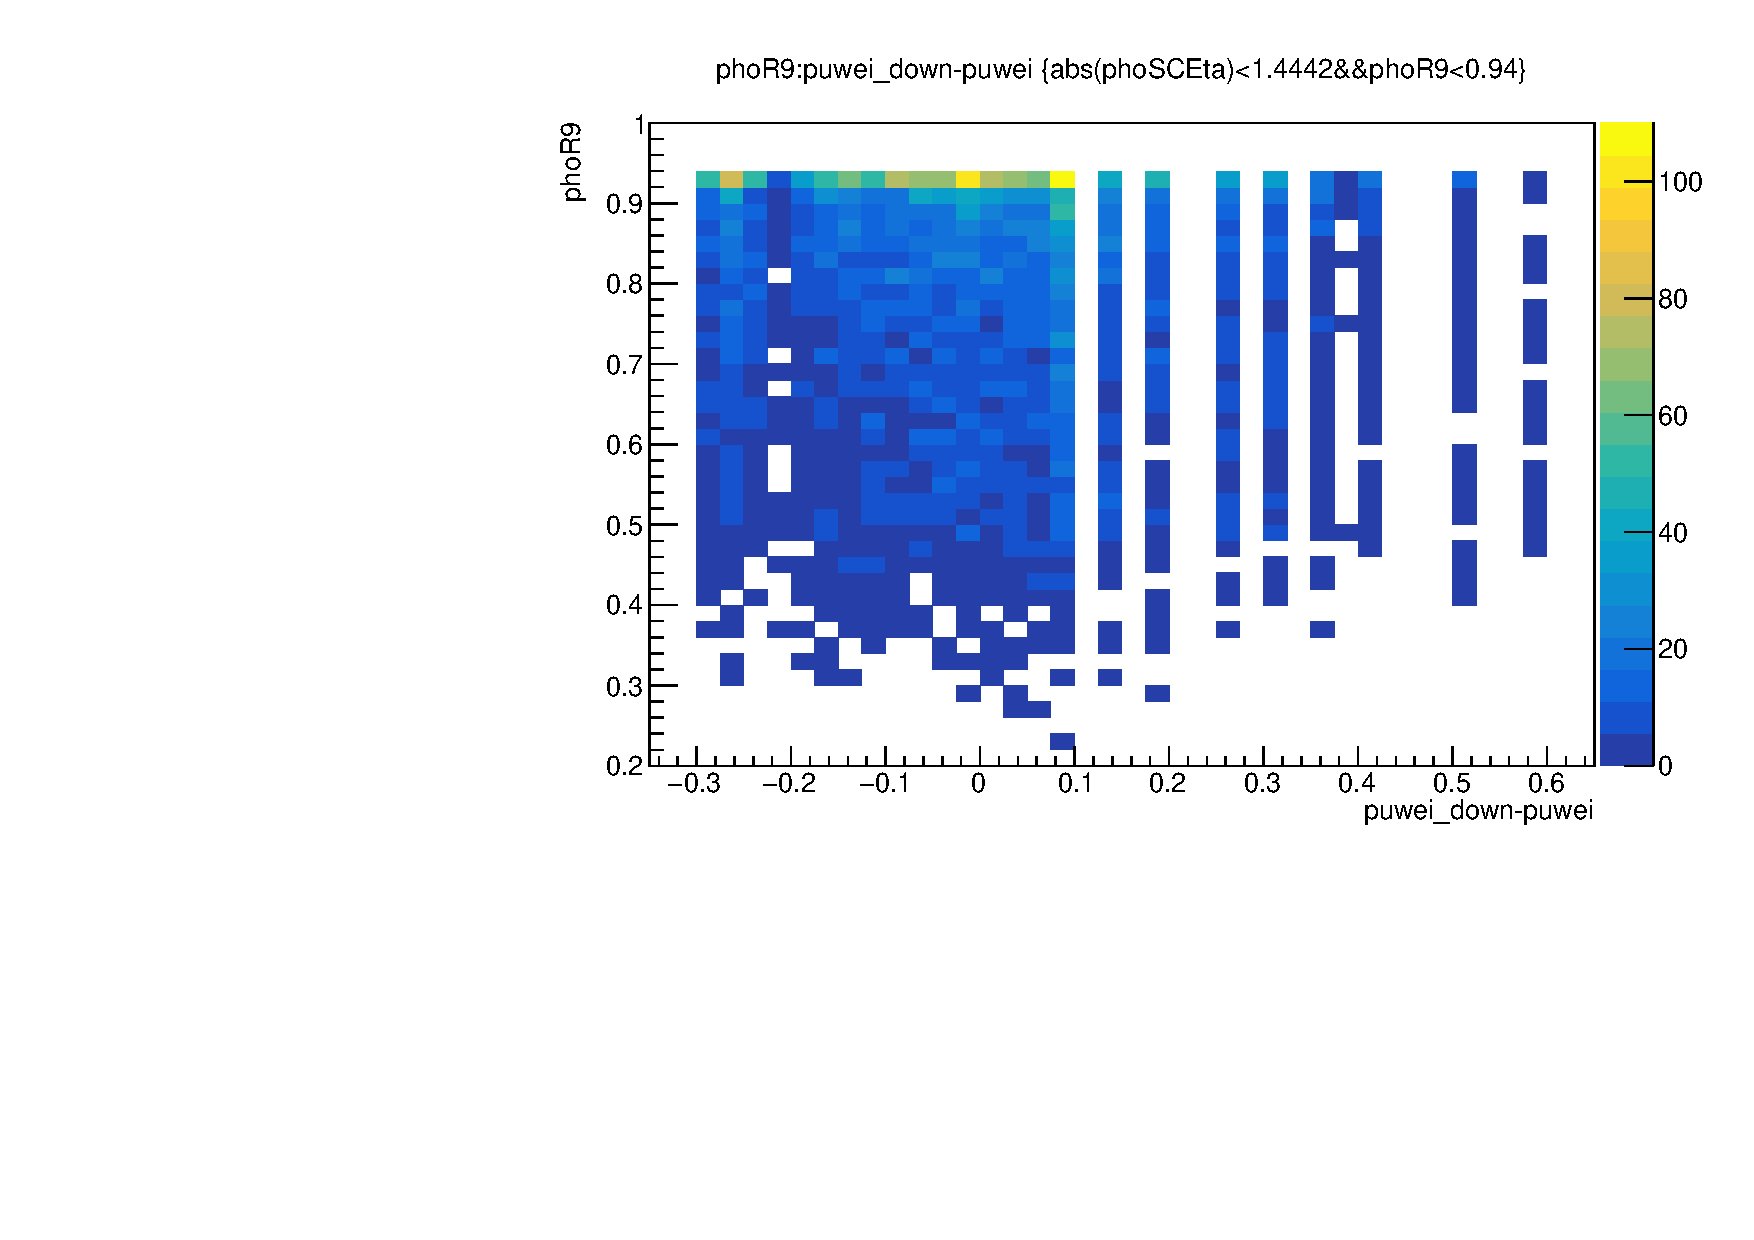
\includegraphics[width=0.50\textwidth]{Fig/puwei_check/phoR9VSpuweidowndiff_EBLR9}\\
	    \bigskip
	    \caption{The 2D distributions of the difference between the up(down) variation and the nominal pile-up weight versus the photon $\RNINE$ value. (Top left) (puwei\_up - puwei) v.s photon $\RNINE$ in EBHR9; (Top right) (puwei\_down - puwei) v.s photon $\RNINE$ in EBHR9; (Bottom left) (puwei\_up - puwei) v.s photon $\RNINE$ in EBLR9; (Bottom right) (puwei\_down - puwei) v.s photon $\RNINE$ in EBLR9}
	  \label{fig:puweidiffvsphoR9}
	  \end{center}
	\end{figure}
	
	\begin{figure}[p]
	  \begin{center}
	    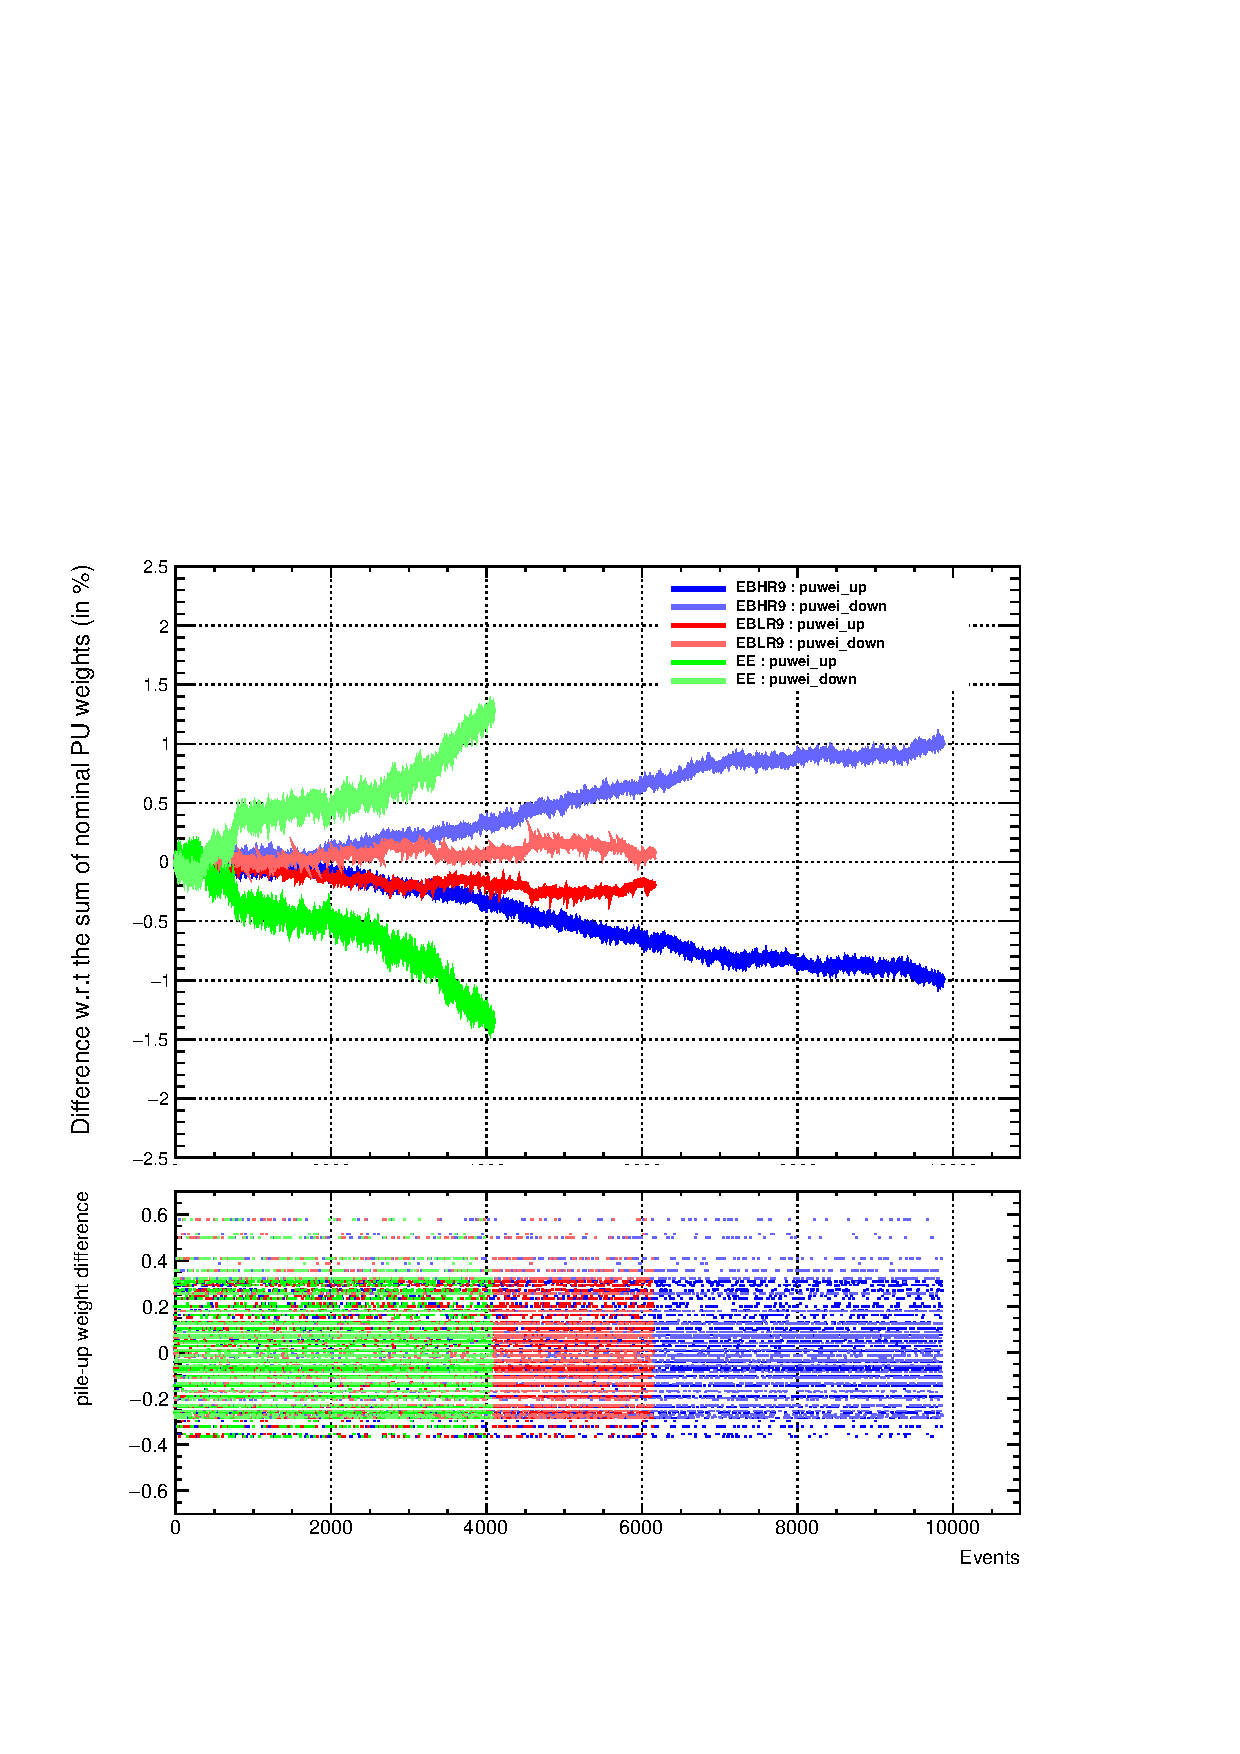
\includegraphics[width=0.9\textwidth]{Fig/puwei_check/puwei_history_root}\\
	    \bigskip
	    \caption{The evolution of the difference with respect to the sum of nominal pile-up weights of all the 3 categories in the Z decay.}
	  \label{fig:puweihistory}
	  \end{center}
	\end{figure}
 
 	 \clearpage
 	 
 \begin{itemize}
	\item \textbf{Muon ID/Isolation}. Muons from $\cPZ$ boson decay are softer than those from the Higgs boson decay, which can be seen in Fig.~\ref{fig:dist-3}, \ref{fig:dist-4}, \ref{fig:dist-5}, \ref{fig:dist-6}. The $\pt$ of muons from the $\cPZ$ boson decay distribute mostly in the range of 20$\sim$30 \GeV, while those from the Higgs boson decay are mostly in the range of 30$\sim$40\GeV, and from the Fig.~\ref{fig:MuonSFs}, one can see that uncertainties in the range of 20$\sim$30 \GeV are slightly higher than those in 30$\sim$40 \GeV. Consequently, uncertainties in muon ID and isolation in the $\cPZ$ boson decay are higher than those in the Higgs boson decay.
	\item \textbf{Electron veto}.  As shown in the Fig.~\ref{fig:PhotonElevetoSFs}, the uncertainty of photons in endcap region is smaller than that of the photon in barrel region by a factor of $0.0044/0.0119=0.37 (37\%)$. The ratio of the uncertainty on the yields in categories of barrel and endcap should be comparable to this number, 0.450/1.200.375 (37.5$\%$). Therefore, the difference of uncertainties between barrel and endcap region is reasonable.
	\item \textbf{Scale uncertainty in the signal modeling}. The individual uncertainty from each source in each category of the Z boson decay is shown in Table~\ref{tab:UnMean}. There are four sets of variation in the muon momentum correction and three sets in the photon energy correction. The final uncertainty in each category are summed in quadrature over the muon and photon part. 
	\item \textbf{Resolution uncertainty in the signal modeling}. The uncertainties in the $\sigma$ of the signal model are larger in the Higgs boson decays than in the $\cPZ$ decay. No unusual behaviors in the distributions of $m_{\mu\mu\gamma}$ resulting from different sets of correction is found, and fits are all reasonable. The difference may come from the correction itself, for which individual analysis cannot do much. The natural width of the $\cPZ$ boson itself is larger, and so relative uncertainty becomes smaller compared to the Higgs boson case. In addition, for the $\cPZ$ decay the first two categories for barrel photons where the uncertainties are smaller, while in Higgs all events are combined and uncertainties from different kinematic regime are averaged. Uncertainties in the muon and photon correction separately are summarized in Table~\ref{tab:HJpsiGUnSigma} and \ref{tab:ZJpsiGUnSigma}. The total uncertainty is derived by summing the uncertainties in the muon and photon parts in quadrature.
	\end{itemize}
	
	\begin{table}[!ht]
	\scriptsize
	    \begin{center}
	    \caption{The uncertainties in the mean of the signal model from muon and photon correction.}
	    \begin{tabular}{lcccccc}
	    \hline
	    & \multicolumn{2}{c}{Cat1 EBHR9} & \multicolumn{2}{c}{Cat2 EBLR9} & \multicolumn{2}{c}{Cat3 EE} \\
	    \cline{2-7}
	    & Scale & Uncertainty (in \%) & Scale & Uncertainty (in \%) & Scale & Uncertainty (in \%) \\
	      \hline
	      \hline
	      Nominal & 91.002 &  & 90.768 &  & 90.950 & \\
	      Muon - Set1 & 91.004 & 0.00220 & 90.785 & 0.0187 & 90.966 & 0.0176  \\
	      Muon - Set2 & 90.997 & 0.00549 & 90.782 & 0.0154 & 90.961 & 0.0121 \\
	      Muon - Set4 & 90.992 & 0.0110 & 90.785 & 0.0187 & 90.956 & 0.00660 \\
	      Muon - Set5 & 90.997 & 0.00549 & 90.782 & 0.0154 & 90.957 & 0.00770 \\
	      Muon - Total & & 0.0136 & & 0.0343 & & 0.0236 \\
	      \hline
	      Photon - gain up & 90.995& 0.00769 & 90.772 & 0.00441 & 90.995 & 0.00769 \\
	      Photon - gain down & 90.995& 0.00769 & 90.772 & 0.00441 & 90.995 & 0.00769 \\
	      Photon - stat. up & 90.996& 0.00659 & 90.772 & 0.00441 & 91.000 & 0.00220 \\
	      Photon - stat. down & 90.994& 0.00879 & 90.772 & 0.00441 & 90.991 & 0.0121 \\
	      Photon - syst. up & 91.030& 0.0308 & 90.830 & 0.0683 & 91.046 & 0.0484\\
	      Photon - syst. down & 90.960& 0.0462 & 90.713 & 0.0606 & 90.945 & 0.0626 \\
	      Photon - Total & & 0.0476 & & 0.0686 & & 0.0643\\
	      \hline
	      Total uncertainty & & 0.0495 & & 0.0767 & & 0.0685\\
	      \hline
	    \end{tabular}
	    \label{tab:UnMean}
	    \end{center}
	\end{table}
	
	\begin{table}[!ht]
	\small
	    \begin{center}
	    \caption{The uncertainties in the sigma of the signal model from muon and photon correction in the $\PH$ decay. The total uncertainty is derived by summing the uncertainties in the muon and photon parts in quadrature. The numbers in the table are in percentage.}
	    \begin{tabular}{ccccccc}
	    \hline
	    & \multicolumn{5}{c}{$\PH\to (\JPsi)\gamma$} \\
	    & ggF & VBF & $\cPZ\PH$ & $\text{W}^{+}\PH$ & $\text{W}^{-}\PH$ & tt$\PH$ \\
	      \cline{2-7}
	      muon &  1.69 & 1.27 & 1.60 & 1.38 & 2.00 & 2.97\\
	      photon & 4.65 & 4.15 & 2.95 & 4.40 & 3.22 & 13.8\\
	      Total & 4.94 & 4.30 & 3.35 & 4.61 & 3.79 & 14.1\\
	      \hline
	    \end{tabular}
	    \label{tab:HJpsiGUnSigma}
	    \end{center}
	\end{table}
	
	\begin{table}[!ht]
	\small
	    \begin{center}
	    \caption{The uncertainties in the sigma of the signal model from muon and photon correction in the $\cPZ$ decay. The total uncertainty is derived by summing the uncertainties in the muon and photon parts in quadrature. The numbers in the table are in percentage.}
	    \begin{tabular}{cccc}
	    \hline
	    & \multicolumn{3}{c}{$\cPZ\to (\JPsi)\gamma$} \\
	    & Cat1 & Cat2 & Cat3 \\
	      \cline{2-4}
	      muon  & 0.44 & 0.38 & 0.49 \\
	      photon & 0.89 & 0.57 & 1.37 \\
	      Total & 0.99 & 0.69 & 1.45 \\
	      \hline
	    \end{tabular}
	    \label{tab:ZJpsiGUnSigma}
	    \end{center}
	\end{table}